\begin{figure}[h!]
	\centering
	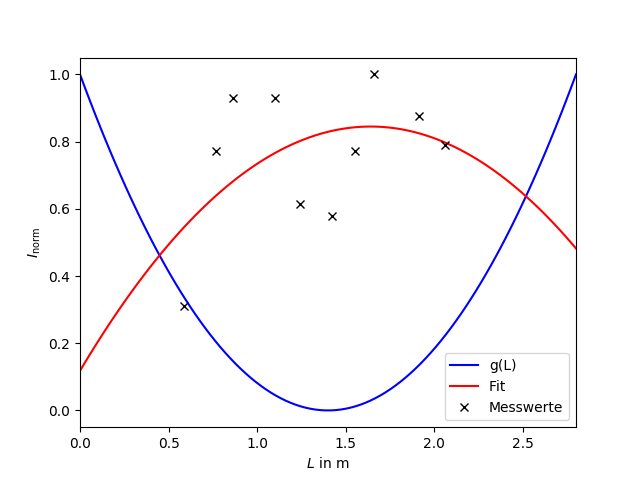
\includegraphics[width=.6\textwidth]{FitCurved.png}
	\caption{Fit zur Überprüfung der Stabilitätsbedingung bei zwei konkaven Spiegeln}
	\label{fig:fitcurved}
\end{figure}
\begin{figure}[h!]
	\centering
	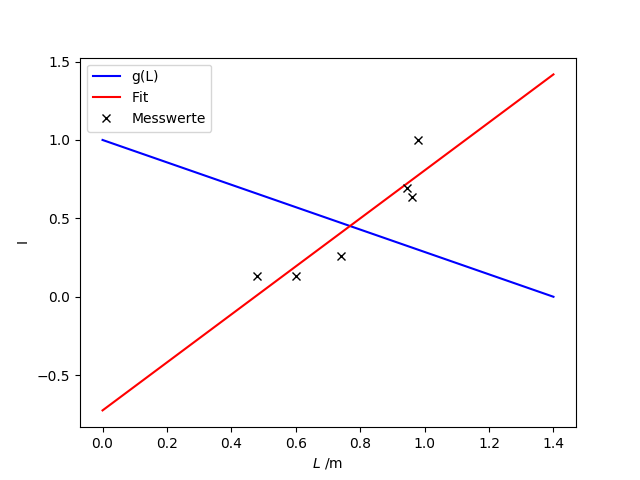
\includegraphics[width=.6\textwidth]{FitFlat.png}
	\caption{Fit zur Überprüfung der Stabilitätsbedingung bei einem gekrümmten und einem flachen Spiegel}
	\label{fig:fitflat}
\end{figure}